\subsection{Vector Bundles}

    \headline{Whitney Sums}

    Given vector bundles $E_1, E_2$ over the same base $B$, we can define their \textbf{Whitney Sum} $E_1 \oplus E_2$ using Theorem \ref{thm:fiber_bundle_construction2} as the vector bundle whose fibers are given by $E_1|_p \oplus E_2|_p$ with the obvious choice as local trivialisations. The following Lemma characterizes the Whitney sum and at the same time provides the technical grounds for an intuition.

    \begin{lemma}[Characterisation of the Whitney sum]
        \label{lem:whitney_sum}
        Let $E_1$ and $E_2$ be vector bundles over the same base space $B$ of rank $k_1$ and $k_2$ respectively. A rank $k_1+k_2$ vector bundle $E$ over $B$ is isomorphic to $E_1 \oplus E_2$ if and only if $E_1$ and $E_2$ can be embedded into $E$ as subbundles and $E_1|_p + E_2|_p = E|_p$ for all $p \in B$.
    \end{lemma}

    Let us first clarify what we mean by embedding. A vector bundle homomorphism $F \colon E \to E^\prime$ is called and \textbf{embedding}, if it is injective. Then $\mathrm{im}(F)$ is a subbundle of $E^\prime$ and $F \colon E \to \mathrm{im}(F)$ is a vector bundle isomorphism. This follows from \cite{lee2011smooth} Theorem 10.34 and Prop. 10.26.

    \begin{proof}[Proof of Lemma \ref{lem:whitney_sum}]
        First let $E = E_1 \oplus E_2$. Then we can define embeddings by
        \[
        F_1 \colon E_1 \to E, \; v \mapsto (v,0),
        F_2 \colon E_2 \to E \; w \mapsto (0,w).
        \]
        Now let $E_1,E_2 \subseteq E$ be subbundles. Let $(U_\alpha)_\alpha$ be an open cover of $B$, such that $E_1$ and $E_2$ are trivial over $U_\alpha$. Choose local frames
        \[
        \sigma^i_{\alpha,1},\ldots, \sigma^i_{\alpha,k_i} \colon U_\alpha \to E_i
        \]
        and define local trivialisations
        \[
        \phi_\alpha^i \colon U_\alpha \times \R^{k_i} \to E_i, \; (p,v) \mapsto \sum_{j=1}^{k_i} v_j \sigma^i_{\alpha,j}(p).
        \]
        Let $\tau^i_{\alpha,\beta} \colon U_\alpha \cap U_\beta \to \mathrm{GL}(k_i)$ be the transition functions defined by
        \[
        ((\phi_\alpha^i)^{-1} \circ \phi_\beta^i)(p,v) = (p,\tau_{\alpha,\beta}^i(p) \cdot v).
        \]
        Since $E|_p$ is the direct sum of $E_1|_p$ and $E_2|_p$, we get that 
        \[
            \sigma^1_{\alpha,1},\ldots, \sigma^1_{\alpha,k_1}, \sigma^2_{\alpha,1},\ldots, \sigma^2_{\alpha,k_2}
        \]
        is a local frame for $E$, thus defines a local trivialisation by
        \[
        \psi_\alpha \colon U_\alpha \times \R^{k_1} \times \R^{k_2} \to E, \; (p,v,w) \mapsto \phi_\alpha^1(p,v) + \phi_\alpha^2(p,w).
        \]
        Then 
        \[
        (\psi_\alpha^{-1} \circ \psi_\beta)(p,v,w) = (p,\tau^1_{\alpha,\beta}(p) \cdot v, \tau^2_{\alpha,\beta}(p) \cdot w).
        \]
        Note that $E_1 \oplus E_2$ is also trivial over $U_\alpha$ via
        \[
        \varphi_\alpha \colon U_\alpha \times \R^{k_1} \times \R^{k_2} \to E_1 \oplus E_2, \; (p,v,w) \mapsto (\phi_\alpha^1(p,v),\phi_\alpha^2(p,w))
        \]
        and $\varphi_\alpha^{-1} \circ \varphi_\beta = \psi_\alpha^{-1} \circ \psi_\beta$, thus
        \[
        E \cong E_1 \oplus E_2
        \]
        by the uniqueness result in Theorem \ref{thm:fiber_bundle_construction1}.
    \end{proof}
     
    This characterisation gives an intuitive reasoning behind the fact, that the Whitney sum of two Moebius bundles is trivial:


    \begin{figure}[ht]
        \centering
        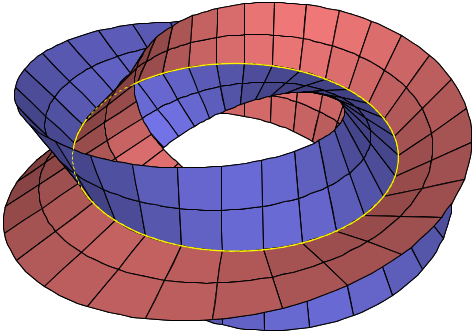
\includegraphics[scale=0.3]{graphics/Whitney_sum_moebius_bundles.png}
        \caption{Illustration of the Whitney sum of two Moebius bundles \small [source: \url{https://math.stackexchange.com/questions/1009126/global-trivialization-of-m-oplus-m}]}
    \end{figure}

    \begin{lemma}
        Let $E, E_1$ and $E_2$ be vector bundles over a manifold $M$ and $\sigma_i \colon M \to E_i$ smooth sections for $i = 1,2$. Then the following maps are smooth:
        \begin{enumerate}[(i)]
            \item $(\sigma_1,\sigma_2) \colon N \to E_1 \oplus E_2, \; p \mapsto (\sigma_1(p),\sigma_2(p))$
            \item The addition map $E \oplus E \to E, \; (v,w) \mapsto v+w$
            \item The scalar multiplication map $\R \times E \to E,\; (\lambda,v) \mapsto \lambda v$
        \end{enumerate}
    \end{lemma}
    \begin{proof}
        All statements follow easily by writing the maps in local trivialisations.
    \end{proof}


    \headline{The Normal Bundle}

    We can generalize Lemma 10.35 from \cite{lee2011smooth} to Riemannian manifolds:

    \begin{lemma}[Orthogonal complement bundles]
        \label{lem:orthogonal_complement_bundles}
        Let $M$ be a Riemannian manifold, $S \subseteq M$ a submanifold and $E \subseteq TM|_S$ a subbundle. Then
        \[
        E^\perp := \{(p,v) \mid p \in S, v \in E_p^\perp\} \subseteq TM|_S
        \]
        is a subbundle and there exists a smooth orthonormal local frame for $E^\perp$ around each point in $S$.
    \end{lemma}
    \begin{proof}
        Choose any local frame 
        \[\sigma_1,\ldots,\sigma_k \colon U \to E.\]
        After possibly shrinking $U$, we can extend this frame to a frame 
        \[\sigma_1,\ldots,\sigma_n \colon U \to TM|_S\]
        of $TM|_S$. Write $\sigma_i(p) = (p,X_p^i)$. Applying Gramm-Schmidt to the vectors $X_p^i$ yields an orthonormal basis $Y_p^1,\ldots,Y_p^n$ of $T_pM$ for each $p \in U$:
        \[Y_p^i := \frac{X_p^i - \sum_{j=1}^{i-1}\langle X_p^i,Y_p^{j} \rangle X_p^i}{\lVert X_p^i - \sum_{j=1}^{i-1}\langle X_p^i,Y_p^{j} \rangle X_p^i \rVert}\]
        Since this formula is smooth, we can define the smooth sections 
        \[\tilde{\sigma}_i(p) := (p,Y_p^i).\]
        Notice that $\tilde{\sigma}_i(p) \in E^\perp$ for $i \geq k+1$ and $E_p^\perp = \mathrm{span}\{Y_p^{k+1},\ldots,Y_p^n\}$. This shows the statement. 
    \end{proof}

    Given a Riemannian manifold $M$ and a submanifold $S \subseteq M$, we can define the \textbf{normal bundle} of $S$:
    \[NS := \{(p,v) \in TM \mid p \in S, v \in T_pS^\perp\}.\]
    \begin{corollary}
        Let $M$ be a Riemannian manifold, $S\subseteq M$ a submanifold. Then $NS$ is a subbundle of $TM|_S$.
    \end{corollary}
    \begin{proof}
        We only need to show, that $TS$ is a smooth subbundle of $TM|_S$ and then apply Lemma \ref{lem:orthogonal_complement_bundles}. To this end, choose a local frame $(\sigma_i)$ of $TS$. Then $\iota \circ \sigma_i$ are sections of $TM|_S$, where $\iota \colon TS \hookrightarrow TM|_S$ is the inclusion. So we only have to verify, that $\iota$ is smooth. But this can easily be seen in local trivialisations of $TS$ and $TM|_S$.
    \end{proof}